\documentclass[submission,copyright,creativecommons]{eptcs}
\providecommand{\event}{ICLP 2022} % Name of the event you are submitting to
\usepackage{breakurl}             % Not needed if you use pdflatex only.
\usepackage{underscore}           % Only needed if you use pdflatex.
\usepackage{amsmath}
\usepackage{amssymb}
\usepackage{xspace}
\usepackage{listings}
\usepackage[inline]{enumitem}
\usepackage[small]{caption}
\usepackage{subcaption}
\usepackage{booktabs}
\usepackage{graphicx}



\newcommand{\jss}{MPF-JSS\xspace}
\title{Solving a Multi-resource Partial-ordering Flexible Variant of the Job-shop Scheduling Problem with Hybrid ASP (Extended Abstract) \thanks{This work was done during an internship of Giulia Francescutto at Infineon Technologies Austria AG and has also been presented at the 17th European Conference on Logics in Artificial Intelligence (JELIA 2021).
Mohammed M.\ S.\ El-Kholany was supported by
KWF project 28472,
cms electronics GmbH,
FunderMax GmbH,
Hirsch Armbänder GmbH,
incubed IT GmbH,
Infineon Technologies Austria AG,
Isovolta AG,
Kostwein Holding GmbH, and
Privatstiftung Kärntner Sparkasse.}}
\author{Giulia Francescutto
\institute{Siemens AG {\"O}sterreich, Vienna, Austria}
\email{giulia.francescutto@siemens.com}
\and
Konstantin Schekotihin
\institute{University of Klagenfurt,
Klagenfurt, Austria}
\email{konstantin.schekotihin@aau.at}
\and
Mohammed M. S. El-Kholany
\institute{University of Klagenfurt, Klagenfurt, Austria}
\institute{Cairo University, Cairo, Egypt}
\email{mohammed.el-kholany@aau.at}
}
%}
\def\titlerunning{Solving MPF-JSS Problem with Hybrid ASP}
\def\authorrunning{G. Francescutto, K. Schekotihin \& M. El-Kholany}
\begin{document}
\maketitle

\begin{abstract}
  In many industries, scheduling is a key component to efficient management of resources and, thus, ensuring competitiveness and success of companies by reducing the consumption of time and money. In this work, we propose a \emph{Multi-resource Partial-ordering Flexible Job-shop Scheduling} % (\jss)
  formulation to capture scheduling scenarios where partially-ordered sequences of operations must be scheduled on multiple required resources, such as tools and specialists.
  The resources are flexible and can process one or more kind of operations based on their characteristics. We have built a model using Answer Set Programming % (ASP) 
  in which the execution time of operations is determined using Difference Logic. Furthermore, we introduced two multi-shot strategies that identify the time bounds and find a schedule while minimizing the total tardiness. 
  Experiments on % a set of 
  instances from an Infineon Fault Analysis lab % provided by a semiconductor manufacturer
  % , and the results showed show 
  show that the proposed model % could find 
  yields schedules for 87 out of 91 real-world instances.
\end{abstract}

\section{Introduction}
% Scheduling systems play an essential role in the success of manufacturing processes, transportation, or cloud computing. Inefficient management of resources results in costly delays and waste of expensive machinery.
Job-shop Scheduling (JSS) \cite{johnson1954optimal} is one of the most well-known scheduling problems in which a set of machines are used to execute given jobs, represented as sequences of operations, and the goal is to complete the jobs as soon as possible.
Extensions like flexible \cite{brucker1990job} and multi-resource
\cite{DBLP:journals/eor/Dauzere-PeresRL98} JSS
generalize the allocation of a machine and additional resources for an operation
to suit practical scheduling applications.
% From this generic formulation, several other scheduling problems have been defined by adding extensions with targeted features that have the goal to formalize in the best possible way real-world scheduling scenarios (\cite{brucker1990job}). %Flexible JSS extends the classical (JSS) problem where an operation can be performed by many machines. The flexible JSS is more complicated because the machine to execute an operation should be determined and then decide the sequence of the operations assigned to each machine \cite{brucker1990job}. 
%Increasing the number of resources to operate makes the problem harder where in some plants, machines and engineers are required to execute operations. 

In this work, we consider a \emph{Multi-resource Partial-ordering Flexible JSS} (MPF-JSS) problem, where multiple resources are needed for executing operations, and jobs consist of partially-ordered sequences of operations to be completed.
% Informally, we are given a set of jobs, where each job is described as a partially ordered sequence of operations.
More specifically, we distinguish machines and engineers as two separate sets of resources
required to perform an operation.
Flexibility lies in the choice among several resources with the required skills in each category.
% We consider two sets of resources that are needed to perform operations. This can be imagined as a scenario where an operation requires both an engineer and a particular machine in order to be executed. Moreover, for each operation, there is more than one resource per resource type that can execute it. 
The goal is to determine the best possible execution order and allocation of operations to resources % wrt. to some predefined criteria, like the minimization of 
for minimizing the total tardiness of jobs wrt.\ their deadlines. 

We model the MPF-JSS problem by an encoding in Answer Set Programming (ASP) with Difference Logic (DL) \cite{gebser2016theory} and take advantage of multi-shot solving \cite{gebser2019multi}.
DL constraints allow for compactly expressing timing requirements, avoiding grounding issues that would otherwise be encountered when a feasible schedule necessitates a large number of time points.
By means of multi-shot solving, we implement two strategies to identify upper time bounds on feasible schedules whose tardiness is further subject to minimization.
% in which a given set of jobs, represented as a partially-ordered set of operations, and two sets of resources that can perform many operations. These resources are tools and engineers trained to operate these operations while optimizing a particular criterion such as tardiness. |This work introduces a model based on Answer Set Programming with Difference Logic \cite{gebser2016theory} to provide an efficient schedule for solving MPF-JSS problem. We suggested applying two different strategies based on the multi-shot solving technique \cite{gebser2019multi} which allows identifying an upper bound on the schedule. 
We tested our proposed model on a dataset representing ten operational days of an Infineon Fault Analysis lab.
Our experiments yield success to obtain schedules for 87 out of 91 real-world instances,
while only a very small number of jobs can be handled without multi-shot solving.
%Each instance represents a whole operational day that was split into smaller instances enabling a detailed assessment of the solving performance. The results showed that obtaining a complete schedule while solving the whole problem in a single shot is impossible. However, applying the multi-shot solving techniques could find schedules for 87 instances out of 91. 

\section{Modeling MPF-JSS with Hybrid ASP}\label{sec:aspmodeling}
We consider a scheduling problem in which different resources are interrelated to process the upcoming operations. In particular, MPF-JSS is an extension of the classical JSS problem where three additional aspects are considered: 
\begin{enumerate*}[label=\emph{(\alph*)}]
	\item \emph{Multi-resources} -- several categories of resources can be required to execute an operation; 
	\item \emph{Partially-ordered} -- some operations cannot be executed before completing their predecessors and others are unaffected by such constraints; and
	\item \emph{Flexible} -- an operation can be performed by a variety of available resources. 
\end{enumerate*}
More specifically, an MPF-JSS instance consists of a set of jobs,
characterized by a partially ordered set of operations to be performed,
where each operation needs to be allocated to some machine and (possibly) an
engineer with the required skills.
The following constraints must be respected:
\begin{enumerate*}[label=\emph{(\roman*)}]
  \item once an operation starts, it cannot be interrupted;
  \item each resource can perform only one operation at a time; 
  \item the execution times of operations of the same job cannot overlap; and
  \item operations must be scheduled according to the partial order given by jobs. % ; and
  % \item the required resources must be available while executing an operation.
\end{enumerate*}



% Answer Set Programming (ASP) modulo Difference Logic (DL) has already been used in the literature to solve scheduling problems and to overcome the grounding issue occurring when dealing with a large number of possible time points (\cite{DBLP:conf/lpnmr/AbelsJOSTW19}). Also, we exploit the power of multi-shot solving to find an upper bound on the tardiness and provide a good starting point for ASP optimization methods. 

We propose two multi-shot ASP modulo DL solving strategies. The first approach incrementally increases the upper bound on the tardiness of each job in order to identify a limit for which schedules are feasible.
%
That is, search starts with the tardiness bound $0$, and if this yields unsatisfiability (UNSAT), the bound is incremented by a constant, 
set by a parameter of our Python control script on top of
\emph{clingo}[DL] \cite{DBLP:journals/tplp/JanhunenKOSWS17},
and this process proceeds until some schedule is found.
% The parameter values are set via a Python control script, which shifts them by the considered window size in each iteration. 
%
Figure~\ref{fig:inc} illustrates an execution of the incremental search strategy, where the bound on jobs' tardiness is increased in steps of size~$2$ until satisfiability (SAT)
is obtained with the time bound~$8$.
ASP optimization methods are then used to find a schedule minimizing the total tardiness, i.e., the
sum of delays over jobs completed after their deadlines.

The second approach performs an exponential binary search for the exact tardiness bound
at which schedules get feasible.
As displayed in Figure~\ref{fig:exp},
the increment on the bound is gradually increased up to step size~$4$ for finding the
first schedule with the time bound~$8$.
A binary search scheme then successively halves the step size for converging to
the exact bound, $7$ in this case, for which schedules are feasible, whose total
tardiness is subject to ASP optimization in the last phase of the multi-shot solving process.
% The second approach finds the upper tardiness bound \lstinline{n} by performing a binary search that exponentially increments \lstinline{n} until the first schedule is identified, and then converges to the smallest \lstinline{n} for which the scheduling problem is still satisfiable (SAT). Figure \ref{fig:exp} illustrates the process converging to the upper bound~$7$, relative to which the tardiness optimization is performed in the second step.

\section{Results}

We conduct our experiments on a set of real-world instances of the \jss problem retrieved from the daily operations history of a semiconductor Fault Analysis (FA) Lab.%  
%
We extracted instances for ten random days representing a snapshot of the situation in the lab. The resulting instances have the following approximate number of fixed components defined by the properties of the studied lab:
\begin{enumerate*}[label=\emph{(\roman*)}]
	\item $50$ operations,
	\item $75$ machines, and 
	\item $45$ workers.
\end{enumerate*}
For each of the days chosen, the number of open jobs ranges between $30$ and $50$. We split each day-instance into sub-instances, with the aim of having instances of increasing size in multiples of $5$, which resulted in a total of $91$ instances.

\begin{figure}
	\begin{minipage}[b]{.5\textwidth}
		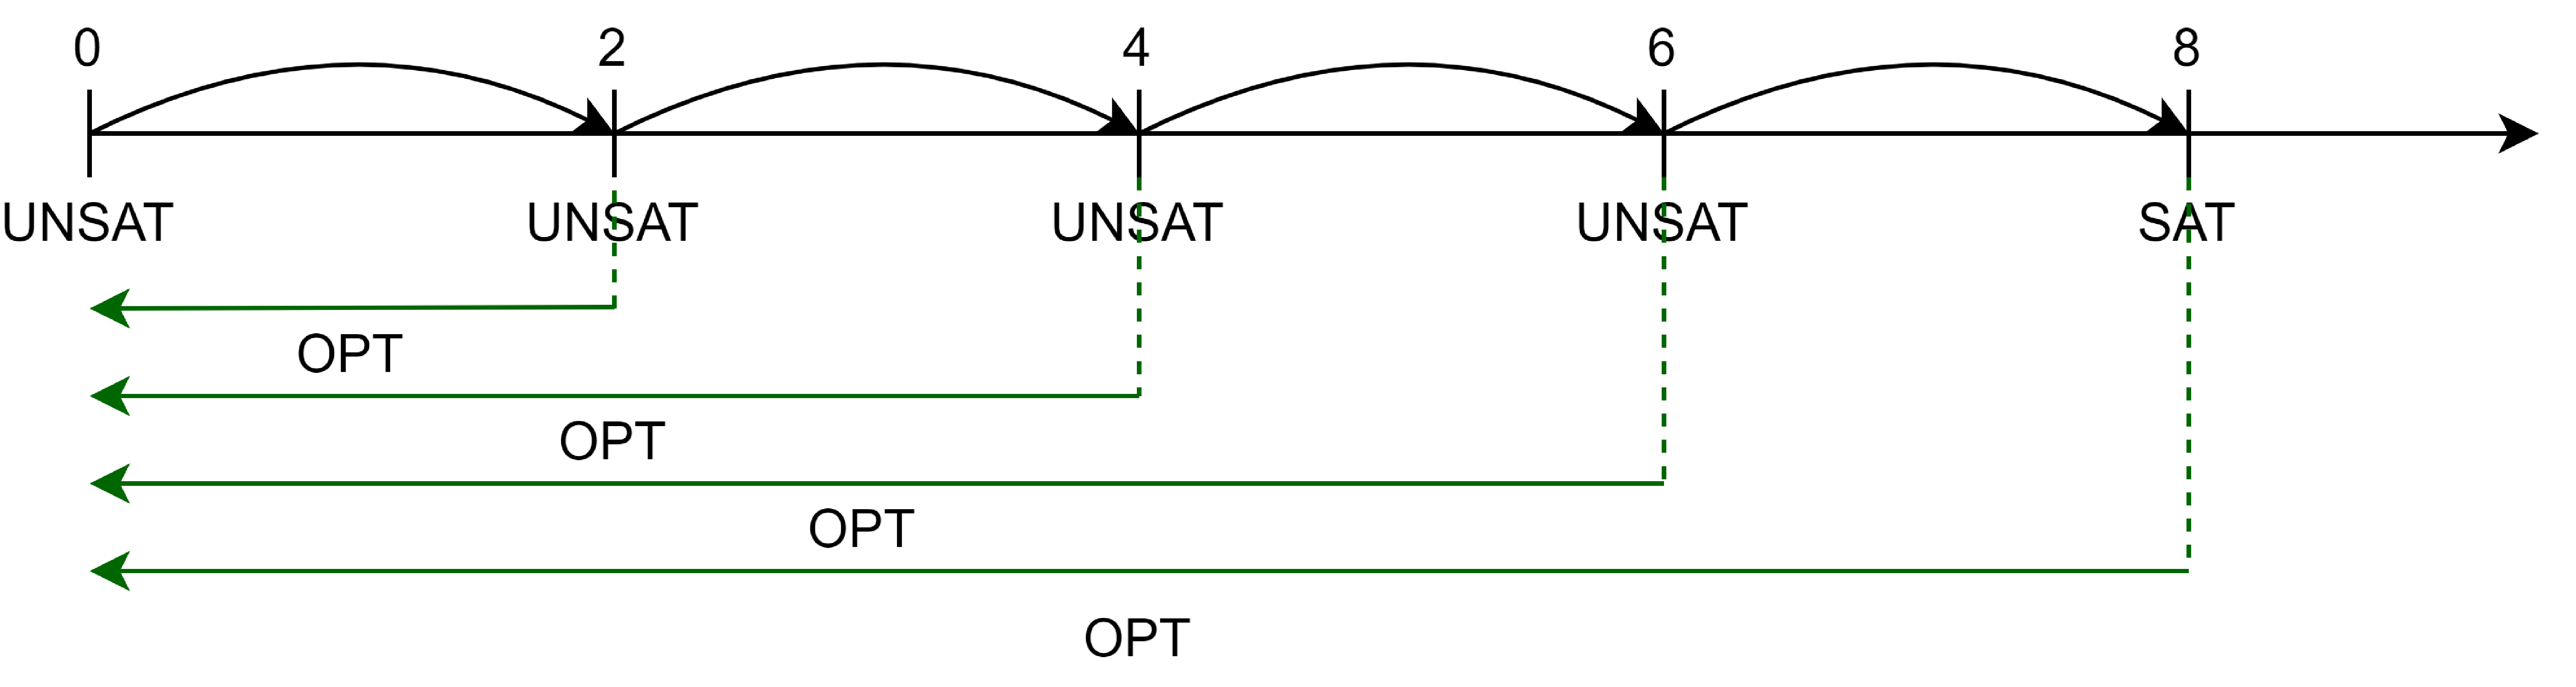
\includegraphics[width=\linewidth]{figures/incremental.pdf}
		\caption{Incremental approach \label{fig:inc}}
			\smallskip %	\vspace{5pt}
			\bigskip
		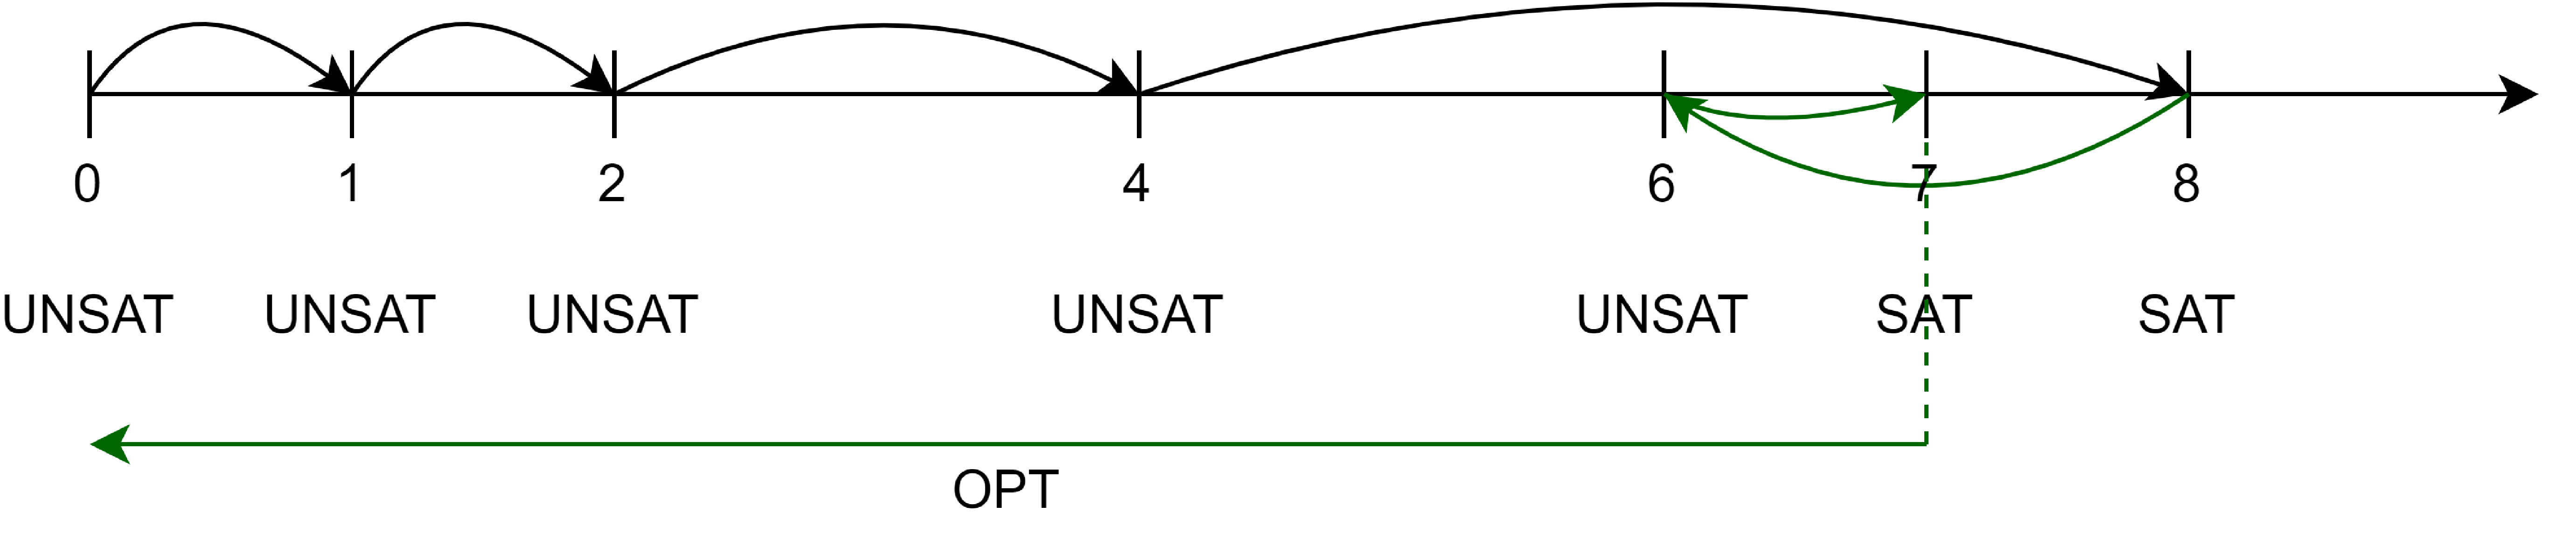
\includegraphics[width=\linewidth]{figures/exponential.pdf}
		\caption{Exponential approach \label{fig:exp}}
	\end{minipage}%
	\begin{minipage}[b]{.5\textwidth}
		\includegraphics[width=\linewidth]{figures/cactus\string_time\string_font20.pdf}
		\caption{Cactus plot of solving times \label{fig:cactus:time}}
	\end{minipage}
\end{figure}

For each obtained instance, we ran three ASP programs: 
\begin{enumerate*}[label=\emph{(\arabic*)}]	
	\item \emph{single-shot} -- base program with a tardiness bound precomputed using a heuristic,
	\item \emph{inc} -- the incremental multi-shot ASP variant, and 
	\item \emph{exp} -- the exponential multi-shot ASP search approach.
\end{enumerate*}
%We compared the multi-shot approaches to a single-shot version where the bound is computed in advance as the sum of durations of all operations in an instance.
%This bound is introduced as a constant in the ASP single-shot program.
The experiments were conducted on a workstation with Ubuntu $18.05$, Intel  $3930$K, and $64$GB RAM. In our experiments, we use \emph{clingo}[DL] 1.1.0 and \emph{clingo} 5.4.0 with multi-shot solving controlled by the main routine in Python 3.8.5. We run the solver up to a timeout of $2$ hours for each instance. For the incremental approach, we chose to use a constant tumbling window of $20$ minutes.

Figure \ref{fig:cactus:time} shows a comparison of the solving performance of the two multi-shot approaches and the single-shot version. The single-shot program reached the timeout for instances with more than $20$ jobs and only managed to find a schedule for instances with $15$ jobs for two days -- Day 2 and Day 9.
%
The two multi-shot approaches significantly outperformed the single-shot version, which reached the timeout for all the instances having more than $20$ jobs. The exponential version solved $87$ instances out of $91$ within the timeout considered, while the incremental version solved $85$ instances. The exponential approach performs slightly better since it always found a tighter upper bound for tardiness, thus, leaving fewer choices for the optimization strategy of the ASP solver. Nevertheless, 
%the differences between the approaches discussed in Section \ref{sec:aspmodeling} were also confirmed in the evaluation. That is, 
in our experiments, the incremental variant was able to obtain better solutions for three instances with an average total tardiness improvement of 80 minutes.

%\section{Conclusions}
%This paper introduces a Multi-resource Partial-ordering Flexible Job-Shop Scheduling (\jss) problem and provides an encoding using ASP modulo DL. The two presented multi-shot solving strategies can find reasonable approximations of tardiness bounds for a set of real-world instances representing daily schedules for a Fault Analysis lab. %Standard single-shot solving could not accomplish the optimization within the same time limit.
%
%In the future, we plan to test the proposed encodings on different problem types to reinforce the assessment. In addition, we aim to devise multi-shot solving strategies with machine learning that can take advantage of historical data, which is often available in industrial application scenarios. 
%In particular, we are going to study combinations of ASP with (supervised) machine learning models trained to guide the search procedure of a solver by giving preference to operations to schedule in successive solving steps. 

%\nocite{*}
\bibliographystyle{eptcs}
\bibliography{generic}
\end{document}
